
\subsection{Three-Dimensional Pressure Prediction and Spatial Error Analysis}
\label{subsec:pressure-spatial-errors}


Figure~\ref{fig:cp-spatial-error-map} shows the spatial distribution of surface-pressure prediction errors at $N=20$, evaluated across the validation wings. For M0, relatively large errors are concentrated on the upper surface, particularly over the forward and midchord portions of the outboard wing. Introducing sectional pressure knowledge reduces these errors over a broad area, while M2 further suppresses several localized regions of high error. The lower-surface errors are generally smaller, consistent with the spanwise error distributions presented in Fig.~\ref{fig:vb_spanwise}. Nevertheless, appreciable errors remain in parts of the outboard upper surface even for M2, indicating that the improvement in pressure prediction is spatially nonuniform.


\begin{figure*}[!t]
    \centering
    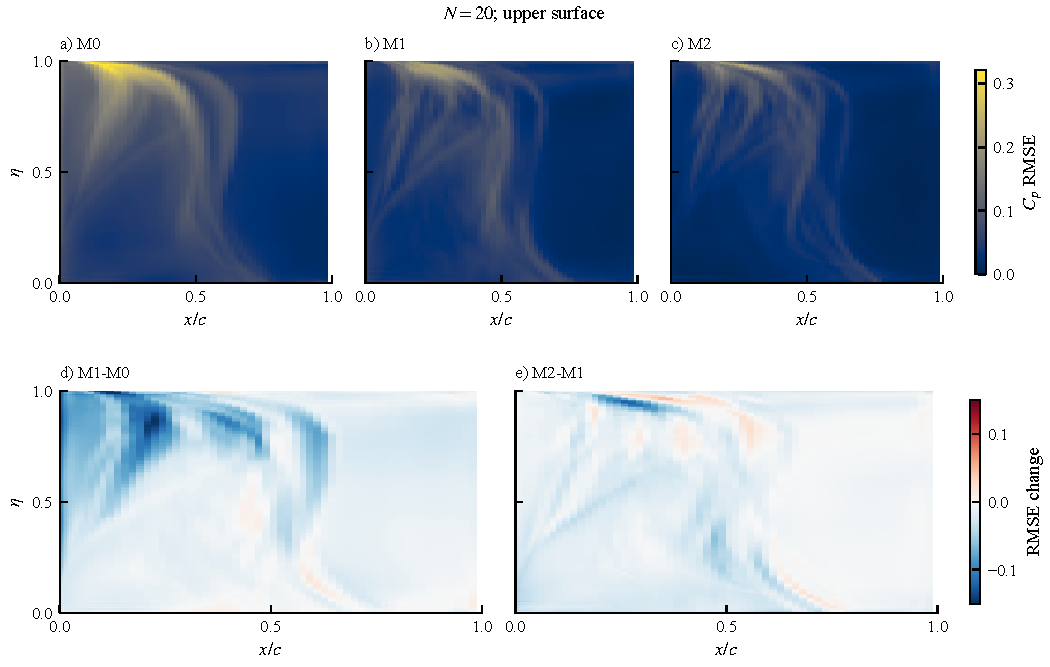
\includegraphics[width=0.93\textwidth]{V_Results_and_Discussion/figures/V_C_Fig18/V_C_Fig18_cp_spatial_error_map.pdf}
    \caption{Upper-surface RMSE maps and differences (M1$-$M0, M2$-$M1) at $N=20$ (41 validation wings; three-run mean). Negative differences indicate error reductions.}
    \label{fig:cp-spatial-error-map}
\end{figure*}

To examine the reconstruction of individual pressure fields, two validation wings with different baseline prediction difficulties are considered. Case A is selected near the median of the wingwise M0 error ranking. As shown in Figs.~\ref{fig:case-a-pressure-field} and \ref{fig:case-a-pressure-sections}, the three models broadly reproduce the spatial pattern of the reference pressure distribution, while M1 and M2 provide improved predictions relative to M0 in several regions of local pressure variation. The chordwise sections further show that the knowledge-based models generally capture the upper- and lower-surface pressure distributions more closely. However, the whole-wing errors of M1 and M2 remain comparable, illustrating that improvements at a small number of representative sections do not necessarily translate into a lower error over the entire wing surface.

\begin{figure*}[!t]
    \centering
    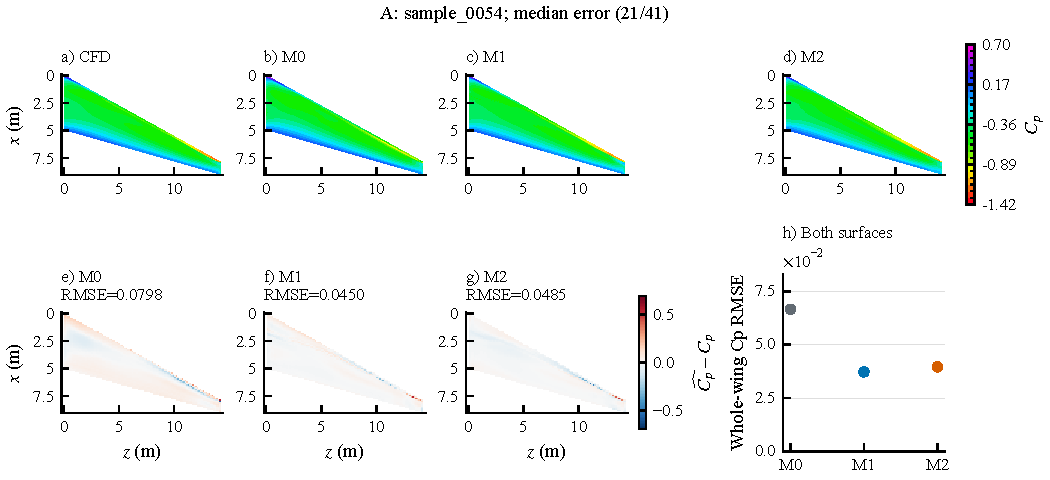
\includegraphics[width=0.93\textwidth]{V_Results_and_Discussion/figures/V_C_Fig19/V_C_Fig19_case_a_pressure_field.pdf}
    \caption{Upper-surface pressure and signed-error fields for Case A ($N=20$), selected near the median M0 RMSE.}
    \label{fig:case-a-pressure-field}
\end{figure*}

\begin{figure*}[!t]
    \centering
    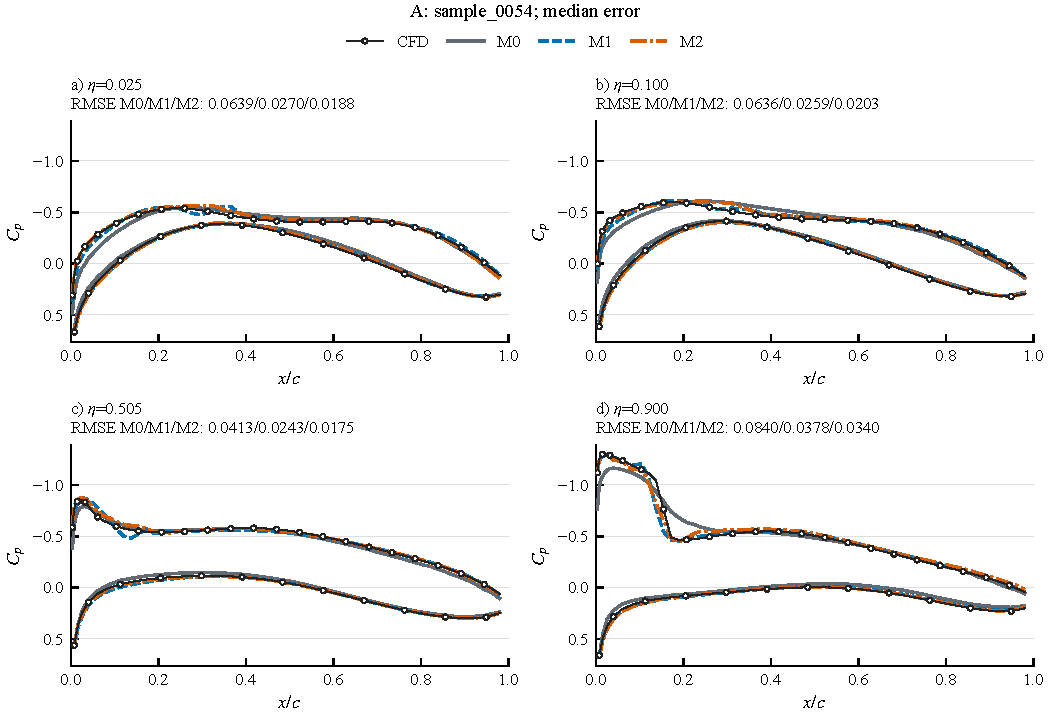
\includegraphics[width=0.93\textwidth]{V_Results_and_Discussion/figures/V_C_Fig20/V_C_Fig20_case_a_pressure_sections.pdf}
    \caption{Chordwise $C_p$ distributions for Case A at four spanwise stations ($N=20$).}
    \label{fig:case-a-pressure-sections}
\end{figure*}

The differences among the knowledge configurations are more pronounced for Case B, which is selected near the 90th percentile of the M0 wingwise error ranking. As shown in Figs.~\ref{fig:case-b-pressure-field} and \ref{fig:case-b-pressure-sections}, the upper-surface pressure distribution exhibits steep pressure recovery over portions of the midspan and outboard wing. M0 and M1 show noticeable discrepancies in the location and shape of these chordwise variations, whereas M2 more closely follows the reference distribution, particularly at outboard stations. At $\eta=0.90$, the sectional RMSE values of M0, M1, and M2 are 0.1520, 0.1476, and 0.0477, respectively. The corresponding whole-wing RMSE values are 0.1092, 0.1024, and 0.0503, demonstrating a substantial improvement in pressure reconstruction for this relatively difficult configuration.

\begin{figure*}[!t]
    \centering
    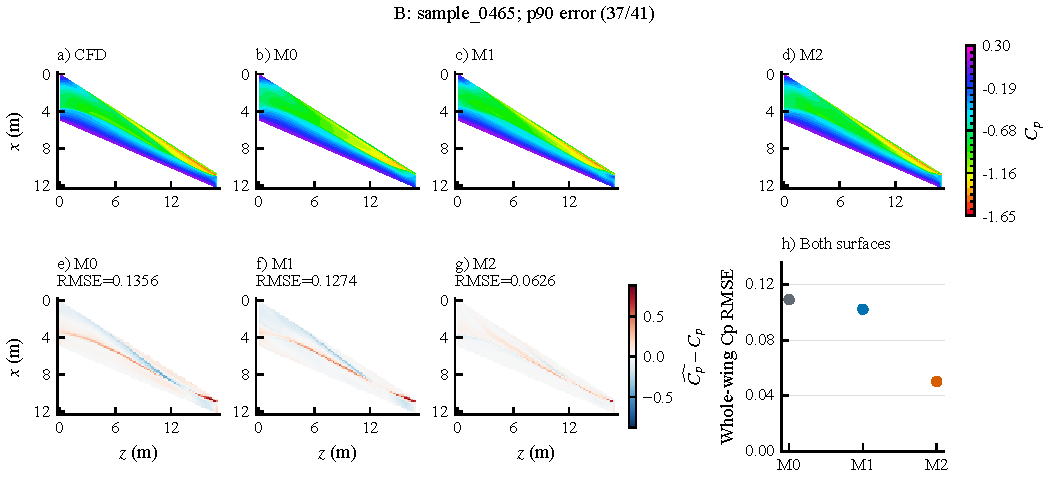
\includegraphics[width=0.93\textwidth]{V_Results_and_Discussion/figures/V_C_Fig21/V_C_Fig21_case_b_pressure_field.pdf}
    \caption{Upper-surface pressure and signed-error fields for Case B ($N=20$), selected near the 90th percentile of the M0 RMSE ranking.}
    \label{fig:case-b-pressure-field}
\end{figure*}

\begin{figure*}[!t]
    \centering
    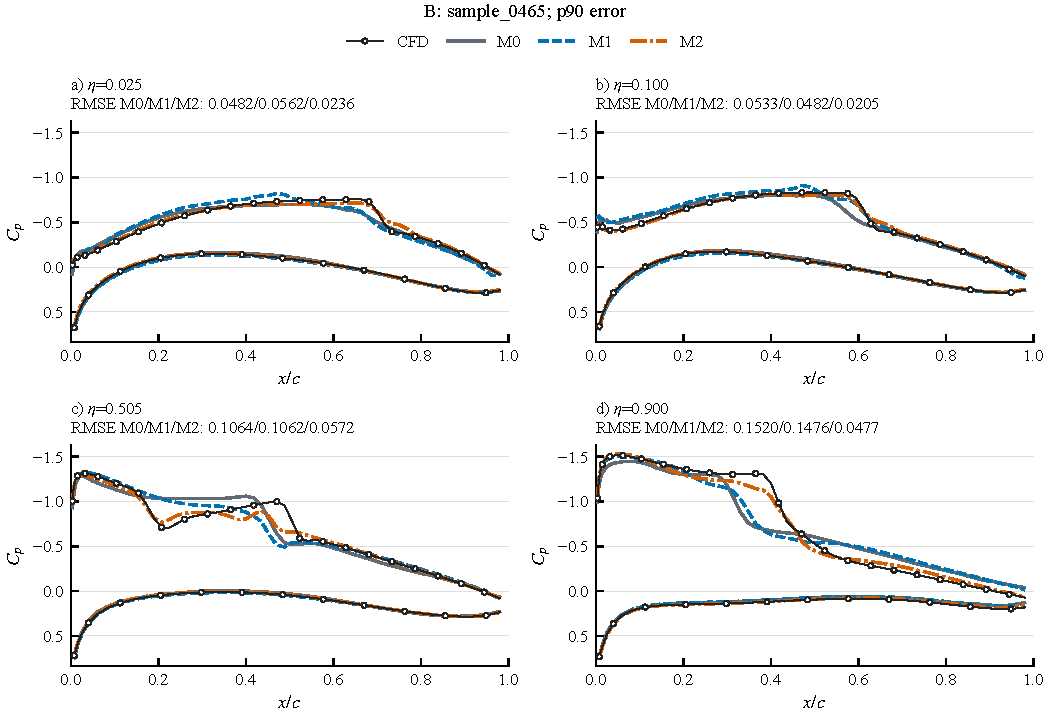
\includegraphics[width=0.93\textwidth]{V_Results_and_Discussion/figures/V_C_Fig22/V_C_Fig22_case_b_pressure_sections.pdf}
    \caption{Chordwise $C_p$ distributions for Case B at four spanwise stations ($N=20$).}
    \label{fig:case-b-pressure-sections}
\end{figure*}

Taken together, the spatial error statistics and representative cases show that hierarchical knowledge transfer improves not only the overall pressure-prediction accuracy but also the reconstruction of certain localized features associated with steep pressure gradients and rapid pressure recovery. The gains nevertheless depend on wing configuration and spanwise location, and noticeable discrepancies persist in some regions of strong pressure variation. The individual cases serve to illustrate these spatial characteristics, whereas conclusions about overall predictive performance are based on the validation-set statistics.
